\chapter{Fields}\label{chapter:fields}

\section{Names for our favourite sets}

The following are the standard names for various collections of numbers (or remainders):
\[
\begin{array}{@{}l>{$}l<{$}@{}}
\Z{} & the set of all integers, \\
\Q{} & the set of all rational numbers, \\
\R{} & the set of all real numbers, \\
\C{} & the set of all complex numbers, \\
m\Z{} & the set of all integer multiples of some number \(m\), \\
\Zmod{m} & the set of remainders modulo a positive integer \(m\).
\end{array}
\]
We can draw \(\R{}\) as the number line, 
\[
\begin{tikzpicture}
\draw[-latex,gray!40](-3,0) -- (3,0);
\end{tikzpicture}
\]
and draw \(\Z{}\) as equispaced dots on the number line,
\[

\begin{tikzpicture}
\draw[-latex,gray!40](-3,0) -- (3,0);
\foreach \i in {-2,...,2}
{
  \fill[gray!30] ({\i},0) circle(1.2pt);
}
\end{tikzpicture}
\]
and \(\C{}\) as the plane:
\[
\begin{tikzpicture}
\draw[-latex,gray!40](-1,0) -- (1,0);
\draw[-latex,gray!40](0,-1) -- (0,1);
\end{tikzpicture}
\]
We could also draw the elements of \(\Zmod{m}\) much like we would draw a clock:
\[
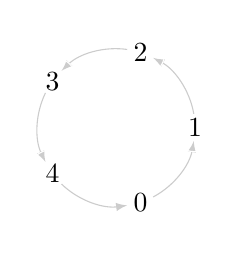
\begin{tikzpicture}
\def \n {5}
\def \nminusone {4}
\def \radius {1cm}
\def \margin {10} % margin in angles, depends on the radius
\foreach \s in {0,...,\nminusone}
{
  \node[draw=white, circle] at ({360/\n * (\s - 1)}:\radius) {$\s$};
  \draw[->, >=latex,gray!40] ({360/\n * (\s - 1)+\margin}:\radius) 
    arc ({360/\n * (\s - 1)+\margin}:{360/\n * (\s)-\margin}:\radius);
}
\end{tikzpicture}
\]

\begin{problem}{rings:pictures}
Explain how to add real numbers, how to add complex numbers, and how to add remainders modulo an integer, using these pictures.
Explain how to multiply complex numbers using these pictures.
\end{problem}


\section{Rings}

All of the above sets are examples of rings.
A \emph{ring}\define{ring} is a set of objects \(S\) together with two operations called \emph{addition} and \emph{multiplication}, and denoted by \(b+c\) and \(bc\), so that if \(b\) and \(c\) belong to \(S\), then \(b+c\) and \(bc\) also belong to \(S\), and so that:
\smallskip
\begin{itemize}
\item[]\emph{Addition laws:}\define{addition laws}
\begin{enumerate}
\item The associative law:\define{associative law!addition} For any elements \(a, b, c\) in \(S\): \((a+b)+c=a+(b+c)\).
\item The identity law:\define{identity law!addition} There is an element \(0\) in \(S\) so that for any element \(a\) in \(S\), \(a+0=a\).
\item The existence of negatives:\define{existence of negatives} for any element \(a\) in \(S\), there is an element \(b\) in \(S\) (denote by the symbol \(-a\)) so that \(a+b=0\).
\item The commutative law:\define{commutative law!addition} For any elements \(b, c\) in \(S\), \(b+c=c+b\).
\end{enumerate}
\smallskip
\item[]\emph{Multiplication laws:}\define{multiplication laws}
\begin{enumerate}
\item The associative law:\define{associative law!multiplication} For any elements \(a, b, c\) in \(S\): \((ab)c=a(bc)\).
\end{enumerate}
\smallskip
\item[]\emph{The distributive law:}\define{distributive law}
\begin{enumerate}
\item For any elements \(a, b, c\) in \(S\): \(a(b+c)=ab+ac\) (left distributive) and \((b+c)a=ba+ca\) (right distributive).
\end{enumerate}
\end{itemize}
\medskip

\begin{example}
Clearly \(\Z{}, \Q{}, \R{}, \C{}\) and \(\Zmod{m}\) (for any positive integer \(m\)) are rings.
\end{example}
\begin{example}
If \(X\) is a set, and \(S\) is a ring, then we can add and multiply any two functions mapping \(X\) to \(S\) by adding and multiplying the values of the functions as usual.
The set \(T\) of all functions mapping \(X\) to \(S\) is a ring.
\end{example}
\begin{example}
If \(S\) is a ring, and \(x\) is an abstract variable (really just a pure symbol that we write down) then a \emph{polynomial}\define{polynomial} in \(x\) with values in \(S\) is a formal expression we write down of the form
\[
a_0 + a_1 x + \dots + a_n x^n
\]
with coefficients \(a_0, a_1, \dots, a_n\) drawn from \(S\).
A polynomial is equal to \(0\) just when all of its coefficients are \(0\).
Denote the set of all polynomials in \(x\) with coefficients from \(S\) as \(S[x]\).
Similarly, if we have two abstract variables \(x\) and \(y\), we treat them as commuting: \(xy=yx\), and then we define \(S[x,y]\) to be the set of all polynomials in \(x\) and \(y\) with coefficients drawn from \(S\).
For example,
\[
\frac{1}{3} - 2x + \frac{4}{7}y + 8 x^2 y + y^3
\]
belongs to \(\Q{}[x,y]\).
\end{example}
\begin{example}
If \(S\) is a ring, a \emph{rational function}\define{rational!function}\define{function!rational} with coefficients drawn from \(S\) is a formal ratio
\[
\frac{b(x)}{c(x)}
\]
of polynomials \(b(x), c(x)\) in \(S[x]\) with \(c(x)\) not the zero polynomial.
We declare such a formal expression to be equal to
\[
\frac{a(x) b(x)}{a(x) c(x)}
\]
for any nonzero polynomial \(a(x)\).
Let \(S(x)\)\Notation{R(x)}{R(x)}{the field of rational functions with coefficients in a ring \(R\)} be the collection of all rational functions with coefficients in \(S\) in a variable \(x\).
\emph{Danger:} even though we call \(\frac{b(x)}{c(x)}\) a \emph{rational function}, it is not, strictly speaking, actually a function, but only a formal expression.
For example, if \(S=\Zmod{2}\), then the rational function
\[
\frac{1}{x(x+1)}
\]
is not defined for any value of \(x\) in \(\Zmod{2}\).
So we have to think of \(x\) not as a variable that varies over some numbers, but as an abstract symbol.
Similarly, a rational function is really not a function but an abstract combination of symbols.
\end{example}
\begin{example}
If \(x,y\) are two abstract variables, we similarly define \(S(x,y)\) to be the ring of all rational functions in \(x,y\), i.e. formal ratios of polynomials in \(x,y\) with coefficients drawn from \(S\).
\end{example}
\begin{example}
If \(R\) is a ring, \(R\left[x,x^{-1}\right]\) means the ring whose elements are \(b(x)+c\of{x^{-1}}\), polynomials in an abstract variable \(x\) and an abstract variable called \(x^{-1}\), but so that when we multiply those two variables together, we get \(1\).
\end{example}
\begin{example}
If \(R\) and \(S\) are rings, let \(R \oplus S\) be the set of all pairs \((r,s)\) where \(r\) is in \(R\) and \(s\) is in \(S\).
Define addition and multiplication by
\begin{align*}
\pr{r_1,s_1} + \pr{r_2,s_2} &\defeq \pr{r_1+r_2,s_1+s_2}, \\
\pr{r_1,s_1} \pr{r_2,s_2} &\defeq \pr{r_1r_2,s_1s_2}.
\end{align*}
Similarly we define a finite (or even an infinite) sum of rings, as the set of finite (or infinite) sequences of elements, one from each ring, with obvious addition and multiplication, element at a time.
\end{example}

\begin{problem}{fields:left.distributive}
Let \(S\) be the set of all polynomials with real coefficients in one variable.
To add elements of \(S\), use usual polynomial addition.
Take the ``multiplication''operation to be composition of polynomials, \emph{not} usual polynomial multiplication.
Prove that \(S\) satisfies all of the laws above, except distributivity, and satisfies left but not right distributivity.
\end{problem}


If a ring \(R\) is a subset of a ring \(S\), and the addition and multiplication operations of \(R\) are just the ones of \(S\) applied to elements of \(R\), then \(R\) is a \emph{subring} of \(S\).
For example, \(\Z{}\) is a subring of \(\Q{}\), which is subring of \(\R{}\), which is a subring of \(\C{}\).



\section{Special types of rings}

A ring is \emph{a ring with identity} if it satisfies
the \emph{identity law}:\define{identity law!multiplication} There is an element \(1\) in \(S\) so that for any element \(a\) in \(S\), \(a1=a\).

A ring is \emph{a division ring} if it satisfies the zero divisors law: for any elements \(a, b\) of \(S\), if \(ab=0\) then \(a=0\) or \(b=0\).

A ring is \emph{commutative} if it satisfies the \emph{commutative law}:\define{commutative law!multiplication} for any elements \(a, b\) of \(S\), \(ab=ba\).
Note that we require \emph{every} ring to have commutative addition; a \emph{commutative} ring is one with commutative multiplication.

The associative law for addition, applied twice, shows that \((a+b)+(c+d)=a+(b+(c+d))\), and so on, so that we can add up any finite sequence, in any order, and get the same result, which we write in this case as \(a+b+c+d\).
A similar story holds for multiplication.

\begin{problem}{fields:matrices}
Let \(S\) be the set of all \(2 \times 2\) matrices with integer coefficients, using the usual laws of matrix addition and multiplication as the addition and multiplication in \(S\).
Prove that \(S\) is a ring with identity, but \emph{not} commutative.
\end{problem}

\begin{problem}{fields:even}
Let \(2\Z{}\) be the set of all even integers using the usual laws of integer addition and multiplication as the addition and multiplication in \(2\Z{}\).
Prove that \(2\Z{}\) is a commutative ring but without identity.
\end{problem}

\begin{problem}{fields:matrices.even}
Let \(2S\) be the set of all \(2 \times 2\) matrices with even integer coefficients, using the usual laws of matrix addition and multiplication as the addition and multiplication in \(2S\).
Prove that \(2S\) is a noncommmutative ring without identity.
\end{problem}

\begin{problem}{rings:zero.equals.one}
Suppose that \(S\) is a ring with identity in which \(0=1\).
Prove that \(S=\set{0}\).
\end{problem}

From here on, we will only be interested in commutative rings with identity.



\section{Fields}

A \emph{unit}\define{unit!ring} in a ring is an element that has a multiplicative inverse, i.e. a reciprocal.
For example, in \(\Zmod{7}\) every nonzero element is a unit, because \(7\) is a prime number.
In \(\Z{}\) the units are \(\pm 1\).
If \(S\) is a ring, we denote by \(S^{\times}\) the set of units of \(S\).
For example, for any ring \(S\), \(\pr{S[x]}^{\times}=S^{\times}\): no polynomial of positive degree has a reciprocal polynomial.
On the other hand, every nonzero rational function is a unit in \(S(x)\): \(\pr{S(x)}^{\times}=S(x)-\set{0}\).

\begin{problem}{fields:units}
Prove that, for any ring \(S\) with identity, if \(b\) and \(c\) are units then \(bc\) is a unit.
\end{problem}

\begin{problem}{rings:zero.divisor.units}
Suppose that \(R\) is a ring and that \(b \in R\) is both a zero divisor and a unit.
Prove that \(R\) has exactly one element, the element zero.
\end{problem}


A \emph{field}\define{field} is a commutative ring with identity, in which every nonzero element is a unit, i.e. has a multiplicative inverse, and in which \(1\ne0\).

\begin{lemma}
For any positive integer \(m\), \(\Zmod{m}\) is a field if and only if \(m\) is prime.
\end{lemma}
\begin{proof}
If \(m\) factors, say as \(m=bc\), with \(b, c\ge 2\), then \(b \ne 0\) modulo \(m\), but \(bc=0\) modulo \(m\), so both \(b\) and \(c\) are zero divisors, and therefore are not units.
If \(m\) does not factor, then \(m\) is prime, and we know that every nonzero element of \(\Zmod{m}\) is a unit; we even have a recipe to find its multiplicative inverse.
\end{proof}

\begin{example}
The set \(\Q{}\) of rational numbers is a field, as is the set \(\R{}\) of real numbers and the set \(\C{}\) of complex numbers.
\end{example}
\begin{example}
Any field \(k\) lies inside the field \(k(x)\) of rational functions with coefficients in \(k\).
In particular, every field is contained inside an infinite field.
\end{example}

We can easily finish the proof of proposition~\vref{proposition:factored.resultants} over any field, because any field \(k\) lies inside an infinite field \(k(x)\).

\begin{problem}{fields:characteristic}
Note that in the field \(k=\Zmod{13}\), we have the peculiar equation \(13=0\).
The \emph{characteristic}\define{characteristic} of a ring with identity \(R\) is the smallest positive integer \(c>0\) so that \(c\) is zero in \(R\) (or in other words, if \(e \in R\) is the identity element, then the element \(c \cdot e = 0 \in R\)).
If there is no such positive number \(c\), we say that \(R\) has characteristic zero.
Prove that the characteristic of a division ring \(R\) is prime, say \(p\), and that there is a unique map \(\Zmod{p} \to R\) which takes \(0\) to \(0\), \(1\) to \(1\), and sums to sums and products to products.
\end{problem}

\begin{problem}{fields:zero.divisors}
A \emph{zero divisor}\define{zero divisor} \(r\) in a ring \(R\) is an element so that \(rs=0\) for some element s of \(R\).
Suppose that \(k\) is a field.
Find the (i) zero divisors and (ii) the units in
\begin{enumerate}
\item \(k\)
\item \(k[x]\)
\item \(k\left[x,x^{-1}\right]\)
\item \(k[x] \oplus k[y]\).
\end{enumerate}
\end{problem}

\begin{example}
Let \(k\) be the set of all real numbers of the form \(a+b2^{1/3}+c2^{2/3}\) for any \(a,b,c\) rational.
Clearly all rational numbers (in particular \(0\) and \(1\)) have this form.
It is easy to check that if add any two such numbers, or subtract, we get another such.
If we multiply two such numbers:
\[
(a+b2^{1/3}+c2^{2/3})(p+q2^{1/3}+r2^{2/3})
=
\alpha + \beta 2^{1/3} + \gamma 2^{2/3}
\]
where
\begin{align*}
\alpha &= ap+2br+2cq, \\
\beta &= aq+bp+2cr, \\
\gamma &= ar+cp+bq.
\end{align*}
We need to check division; this turns out to be difficult.
Associate to each such number \(a+b2^{1/3}+c2^{2/3}\) the vector \((a,b,c)\) in \(\Q{3}\).
The product \((a+b2^{1/3}+c2^{2/3})(p+q2^{1/3}+r2^{2/3})\) has associated vector
\[
\begin{pmatrix}
a & 2c & 2b \\
b & a & 2c \\
c & b & a
\end{pmatrix}
\begin{pmatrix}
p \\
q \\
r
\end{pmatrix}.
\]
The determinant of the matrix
\[
A=
\begin{pmatrix}
a & 2c & 2b \\
b & a & 2c \\
c & b & a
\end{pmatrix}
\]
is \(a^3+2b^3+4c^3-6abc\).
We need to prove that this determinant is nonzero, i.e. that there is an inverse matrix.
Indeed the reader can check that
\[
A^{-1}=
\frac{1}{\det A}
\begin{pmatrix}
\bar{a} & 2\bar{c} & 2\bar{b} \\
\bar{b} & \bar{a} & 2\bar{c} \\
\bar{c} & \bar{b} & \bar{a}
\end{pmatrix}
\]
where \(\bar{a}=a^2-2bc\), \(\bar{b}=2c^2-ab\), \(\bar{c}=b^2-ac\).
Note that this tells us precisely that
\[
\frac{1}{a+b2^{1/3}+c2^{2/3}}
=
\frac{\bar{a}+\bar{b}2^{1/3}+\bar{c}2^{2/3}}{\det A}.
\]

So in order to see that \(k\) is a field, and check the above expression for division in \(k\), we only need to check \(\det A \ne 0\).
In other words, let's check that if \(a,b,c\) are rational numbers, not all zero, then
\(a^3+2b^3+4c^3 \ne 6abc\).
Note that we can rescale all of \(a,b,c\) by the same constant, and both sides of the inequality \(a^3+2b^3+4c^3 \ne 6abc\) scale by the same factor.
So we can scale \(a,b,c\) so that they become coprime integers.
If \(a^3+2b^3+4c^3=6abc\), clearly \(a^3\) is even, so \(a\) is even, say \(a=2\alpha\).
Then \(a^3+2b^3+4c^3=6abc\) becomes \(8\alpha^3+2b^3+4c^3=12\alpha bc\).
Divide out 2 to get \(4\alpha^3+b^3+2c^3=6\alpha bc\).
Clearly \(b\) is even, say \(b=2\beta\); plug in: \(4\alpha^3+8\beta^3+2c^3=12\alpha \beta c\).
Divide out 2 to get \(2\alpha^3+4\beta^3+c^3=6\alpha \beta c\).
Finally we see that \(c\) is even, contradicting the fact that \(a,b,c\) are coprime integers.
Hence we conclude that \(k\) is a field.
\end{example}

\section{Linear algebra}

Most of linear algebra works identically over any field: matrices, Gaussian elimination, invertibility, solvability of equations, determinants, and the theory of eigenvalues and eigenvectors.

\begin{problem}{fields:invert.matrix}%
Let \(k\) be the Boolean numbers \(k\defeq \Zmod{2}\), and \(A\) the
matrix
\[
A =
\begin{pmatrix}
0 & 1 & 0 \\
1 & 0 & 1 \\
1 & 1 & 0
\end{pmatrix},
\]
thought of as having entries from \(k\). Is \(A\) invertible?
If so, find \(A^{-1}\).
\end{problem}

\begin{problem}{fields:rank}
    If \(A\) is a matrix whose entries are rational functions of a
    variable \(t\) over a field \(k\), prove that the rank of \(A\) is constant in \(t\), except for finitely many values of \(t\).
\end{problem}

\begin{problem}{fields:rank.mod.p}
    If \(A\) is a matrix whose entries are integers, let \(A_p\) be the same matrix, but with coefficients taken modulo a prime \(p\).
    Prove that \(A\) is invertible over the rational numbers (i.e. has an inverse matrix with rational number entries) just when, for all but finitely many primes \(p\), the matrix \(A_p\) is invertible over \(\Zmod{p}\).
    Prove that \(A\) is not invertible over the rational numbers just when, for every prime number \(p\), \(A_p\) is not invertible over \(\Zmod{p}\).
    Prove that \(A\) is invertible over the integers just when, for every prime number \(p\), the matrix \(A_p\) is invertible over \(\Zmod{p}\).
\end{problem}



